% \chapter{Структура КХЭД} \label{chapt2}
\subsection{Структура КХЭД} \label{storage}
% \addcontentsline{toc}{chapter}{Структура КХЭД}  % Добавляем его в оглавление

На рис. \ref{img:uml} изображена схема описанных модулей в нотациях UML.

% \begin{figure} [h] 
%   \center
%   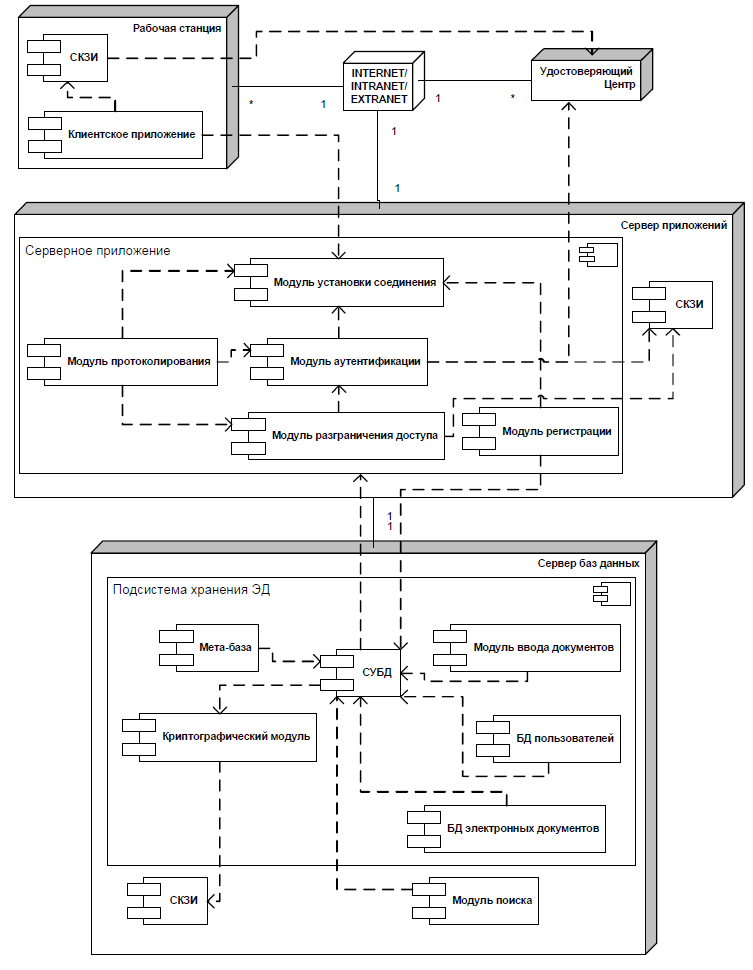
\includegraphics [scale=0.6] {uml.png}
%   \caption{Структура КХЭД} 
%   \label{img:uml}  
% \end{figure}
\begin{figure}[p]
  \centering
  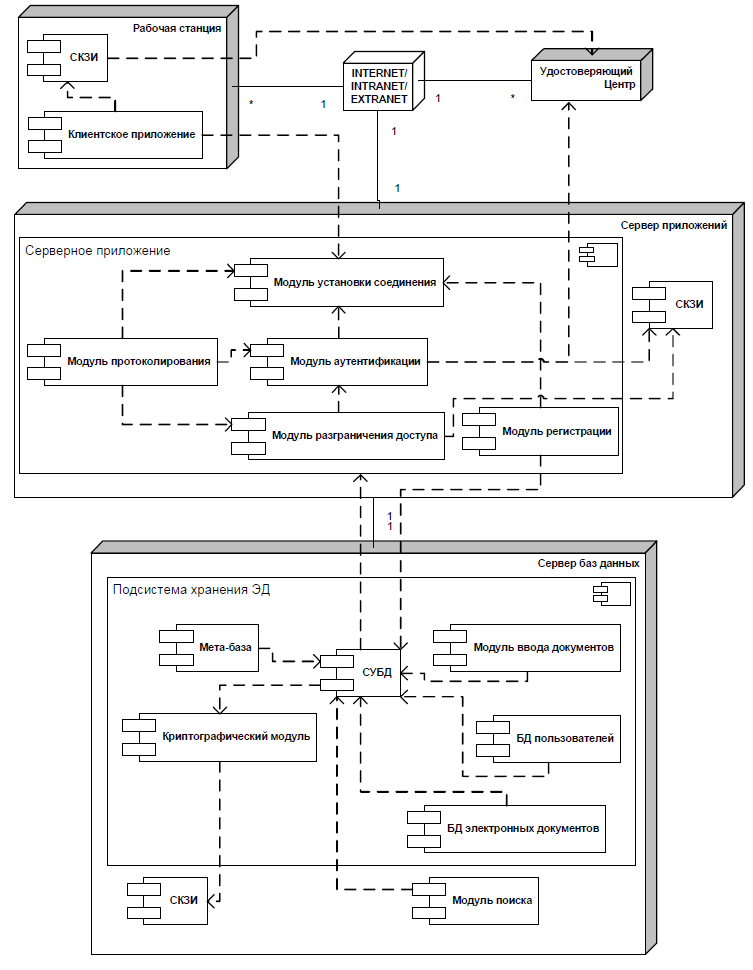
\includegraphics[width=1\textwidth]{uml}
  \caption{Структура КХЭД}
  \label{img:uml}
\end{figure}

\begin{itemize}
\item Модуль установки соединения

Отвечает за организацию процесса подключения пользователя к конфиденциальному хранилищу электронных документов и передачу данных -- проведение процедуры согласования параметров соединения, помещение заявок пользователей на ожидание в очередь основного процесса сервера приложений, выделение параллельных потоков для работы пользователя с системой.

\item Модуль аутентификации

Отвечает за проверку принадлежности субъекту доступа предъявленного им идентификатора.

\item Модуль разграничения доступа

Предназначен для проверки прав пользователей на доступ к функциям системы и электронным документам, а также для ограничения и контроля действий пользователей в соответствии с их правами.

\item Модуль хранения электронных документов

Отвечает за организацию конфиденциального хранения электронных документов и за предоставление доступа к ним пользователей.

\item Модуль поиска и редактирования

Предназначен для осуществления поиска ЭД по запросам пользователей, а также внесения изменений в них.

\end{itemize}
% \clearpage